\section{Materials and methods}
Fig.~\ref{fig:pipeline} and Algorithm~\ref{alg:pipeline} give an overview of the method. Only the N3 detector is learned; every score for detected epochs is a fixed rule applied to the signal.

\begin{figure*}[!t]
\centering
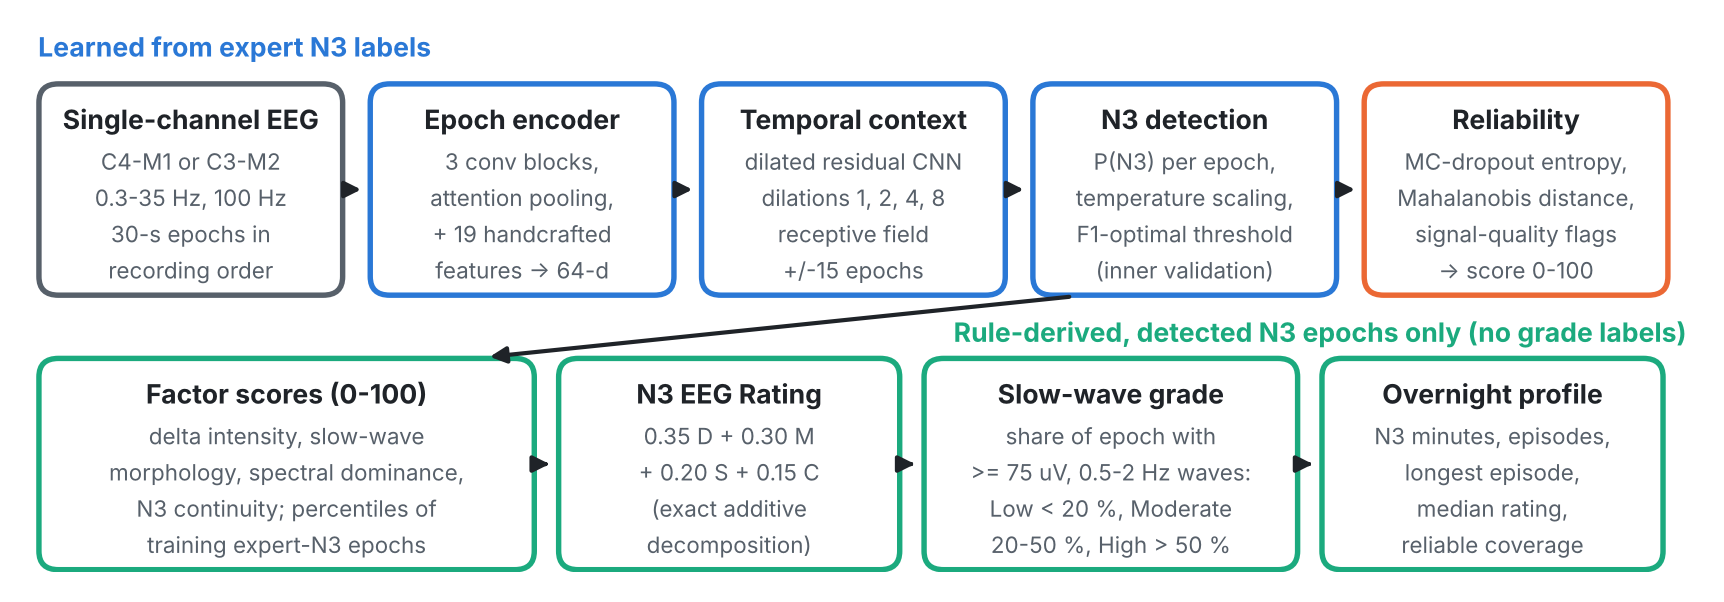
\includegraphics[width=0.62\textwidth]{fig_pipeline.png}
\caption{Overview. Top row: the detector is trained on expert N3 labels and gives a temperature-scaled N3 probability for each 30-s epoch; a separate reliability model combines model confidence, out-of-distribution distance and signal-quality flags. Bottom row: for epochs detected as N3, fixed rules calculate four factor scores and their additive rating and assign a three-level slow-wave grade; nightly summaries form an overnight profile. No grade or quality labels are used at any step.}
\label{fig:pipeline}
\end{figure*}

\subsection{Cohorts}
Table~\ref{tab:cohorts} lists the seven cohorts. ISRUC-Sleep subgroup I (100 adults recorded at a clinical sleep centre, two scorers) and the Haaglanden Medisch Centrum database (151 clinical recordings, one technician, AASM version 2.4) were the training cohorts \cite{khalighi2016isruc,alvarez2022hmcdb,alvarez2021hmc}. The other five cohorts were used only for testing: ISRUC-Sleep subgroup II (eight participants recorded twice, used for test--retest analysis), subgroup III (ten healthy participants) \cite{khalighi2016isruc}, the Dreem Open Datasets DOD-H (25 healthy volunteers) and DOD-O (55 patients with obstructive sleep apnea), each scored by five technicians from different centres \cite{guillot2020dod}, and the CAP Sleep Database (108 recordings scored with the Rechtschaffen and Kales rules, stage 3 and stage 4 separate) \cite{terzano2001cap,goldberger2000physionet}. CAP served only as the expert stage 3/4 reference for the slow-wave grade and for reporting detection; it is not part of the external criterion of the detection analysis. In total, the data contained 465 recordings, 437,430 epochs and 457 participants. % E: data_inventory.csv, run notebook cell 28 (465, 437430, 457)

For ISRUC, the reference label comes from the first scorer, and the second scorer is used only for inter-rater analyses. For DOD, the reference label is the majority vote of the five scorers; ties are broken by the scorer with the highest mean agreement \cite{guillot2020dod}. The public DOD-O signals are cropped at the start relative to the scorer hypnograms of the evaluation repository. We therefore matched the scorer consensus to the hypnogram stored in each DOD record, which is aligned with that record's signal, by choosing the epoch offset that maximised their agreement. This step uses labels only. All 80 records were matched (median offset 106 epochs in DOD-O; agreement at least 0.847); records with agreement below 0.6 would have been excluded. We found this misalignment after the first full run, and all reported results use the matched labels, with no change to the criteria or model settings. Because the matching depends on labels, its possible effect on the DOD results has not yet been checked with a label-free alignment (Section~\ref{sec:limitations}). % E: ledger_extra 80, 106, 0.847; methods_parameters.csv DOD reference

\begin{table}[!t]
\caption{Cohorts. Epochs are expert-scored 30-s epochs; N3 is the share of scored epochs in the evaluated set. Native rates were resampled to 100~Hz.}
\label{tab:cohorts}
\centering
\setlength{\tabcolsep}{3pt}
\footnotesize
\begin{tabular}{@{}llrrrrl@{}}
\toprule
Cohort & Role & Part. & Rec. & Epochs & N3 & Channel (native Hz) \\
\midrule
ISRUC-I & training & 100 & 100 & 90,187 & 0.194 & C4-M1 (200) \\ % data_inventory, rq1_detection_metrics cohort=ISRUC-I
HMC & training & 151 & 151 & 137,243 & 0.194 & C4-M1 (256) \\
ISRUC-II & external, retest & 8 & 16 & 14,207 & 0.184 & C4-M1 (200) \\
ISRUC-III & external & 10 & 10 & 8,889 & 0.229 & C4-A1 (200) \\
DOD-H & external, 5 scorers & 25 & 25 & 24,665 & 0.140 & C3-M2 (250) \\
DOD-O & external, 5 scorers & 55 & 55 & 53,236 & 0.105 & C4-M1 (250) \\
CAP & S3/S4 reference & 108 & 108 & 107,976 & 0.239$^{a}$ & C4-A1$^{b}$ (100--512) \\
\bottomrule
\end{tabular}
\vspace{2pt}

\raggedright\scriptsize HMC, Haaglanden Medisch Centrum; DOD, Dreem Open Datasets; Part., participants; Rec., recordings. A1 and M1 denote the same mastoid reference; ISRUC-I and ISRUC-II contain both labels. $^{a}$R\&K stage 3 + 4 share in the 105 evaluated recordings (three excluded, Section~\ref{sec:exclusions}). $^{b}$104 recordings C4-A1, four C3-A2. Age (mean $\pm$ SD) and sex from the source releases: HMC 53.9 $\pm$ 15.4 years, 85 men/66 women (151 recordings of release 1.1) \cite{alvarez2022hmcdb}; DOD-H 35.3 $\pm$ 7.5, 19/6; DOD-O 45.6 $\pm$ 16.5, 35/20 \cite{guillot2020dod}; CAP 44.8 $\pm$ 19.5, 62/40 (102 with age); ISRUC demographics were no longer retrievable.
\end{table}

\subsection{Signal processing}
\label{sec:exclusions}
From each recording we used one central derivation, C4-M1 (or C4-A1, which has the same mastoid reference), or otherwise C3-M2; no other channel was ever used instead. One ISRUC-I recording stored monopolar channels and was re-referenced as C4$-$A1. Signals were band-pass filtered at 0.3--35~Hz (fourth-order zero-phase Butterworth), resampled to 100~Hz and cut into 30-s epochs (3,000 samples) in recording order. All scored epochs were kept; quality-control flags (amplitude, z-score, high-frequency power, clipping) were stored but never used to remove epochs. Three CAP recordings contained values outside the range of the 16-bit floating-point cache. They were excluded from all evaluations by a model-independent rule (non-finite cached signal), which we identified during the first analysis run and applied in the same way to all models. % methods_parameters.csv; evaluation_exclusions.csv (CAP n13-n15)

For each epoch we computed nineteen handcrafted features from a Welch spectrum (4-s Hann windows, 50\% overlap): absolute and relative power in the slow-delta (0.5--2~Hz), delta (0.5--4~Hz), theta, alpha, sigma and beta bands, delta/theta, delta/alpha and delta/beta log-ratios, spectral entropy, and slow-wave measures from a zero-crossing full-wave detector \cite{massimini2004travelling} (0.3--4~Hz band-pass; negative half-wave 0.25--1.0~s; full wave 0.5--2.0~s): wave count per minute, the share of the epoch covered by waves of at least 75~\textmu V, and the median peak-to-peak amplitude and ascending slope of candidate waves. The features were standardised with the median and interquartile range of the training fold and clipped at $\pm$10 interquartile ranges.

\begin{algorithm}[!t]
\caption{Detection and description of one recording}
\label{alg:pipeline}
\footnotesize
\begin{algorithmic}[1]
\Require one central EEG channel $x$; fold models $f_k$ with thresholds $\tau_k$ and temperatures $T_k$; training reference $\mathcal{R}$ (expert N3 epochs); reliability model $g$
\Ensure per epoch: label $\hat{y}_i$, probability $p_i$, scores $D_i, M_i, S_i, C_i$, rating $R_i$, grade, reliability $r_i$; overnight profile
\State $x \gets$ band-pass 0.3--35~Hz, resample to 100~Hz, cut into 30-s epochs $e_1,\dots,e_N$
\State $z_i \gets e_i / \mathrm{median}_j\,\mathrm{SD}(e_j)$; \ $h_i \gets$ 19 spectral and slow-wave features of $e_i$
\For{each model $f_k$ (test-fold model in CV; all five externally)}
  \State $u_i \gets W[\mathrm{AttnPool}(\mathrm{CNN}(z_i)) \,\|\, h_i]$ \Comment{64-d epoch embedding}
  \State $v_{1:N} \gets \mathrm{DilatedConv}_{d=1,2,4,8}(u_{1:N})$ \Comment{$\pm$15 epochs}
  \State $\ell^k_i \gets \mathrm{Head}(v_i)$
\EndFor
\State $\hat{y}_i \gets [\,\overline{\sigma(\ell^k_i)} \ge \overline{\tau_k}\,]$; \ $p_i \gets \overline{\sigma(\ell^k_i/T_k)}$ \Comment{mean over models}
\ForAll{$i$ with $\hat{y}_i = 1$}
  \State $D_i, M_i, S_i \gets$ mean percentile of their metrics in $\mathcal{R}$
  \State $C_i \gets 100 \cdot \mathrm{mean}(\hat{y}_{i-5},\dots,\hat{y}_{i+5})$
  \State $R_i \gets 0.35D_i + 0.30M_i + 0.20S_i + 0.15C_i$
  \State grade $\gets$ Low / Moderate / High for coverage $<$20\%, 20--50\%, $>$50\%
\EndFor
\State $r_i \gets 100\,g(\max(p_i,1-p_i), \text{MC entropy}, \text{MI}, \text{Mahalanobis}, \text{QC})$
\State episodes $\gets$ runs of $\ge 2$ detected epochs, gaps $\le 2$ merged; profile $\gets$ N3 minutes, episodes, median $R$
\end{algorithmic}
\end{algorithm}

\subsection{Detection network}
The epoch encoder has three convolutional blocks (16, 32 and 48 channels, kernels 32, 16 and 8 samples, batch and layer normalisation) followed by additive attention pooling over 32 time steps. The 48-dimensional output is joined with the 19 features and projected to a 64-dimensional embedding. A residual temporal block of four dilated convolutions (kernel 3, dilations 1, 2, 4 and 8) then combines the embeddings of neighbouring epochs, which gives a receptive field of $\pm$15 epochs (7.5~min). Finally, a two-layer head gives one N3 logit per epoch. The network has 96,226 parameters. % rq1_sota_comparison n_params

\subsection{Training and evaluation protocol}
We trained with participant-grouped five-fold cross-validation on ISRUC-I and HMC, stratified by cohort. In each training fold, 15\% of the participants of each cohort formed an inner validation set. The outer test fold was never used for any decision: early stopping (inner precision--recall area, patience 5, at most 30 passes), temperature scaling \cite{guo2017calibration} and the decision threshold (maximum inner F1 score) were all based on the inner set. The folds were fixed at the first training session, and before the analysis we checked that every saved run matched the evaluated cache exactly (97 of 97 runs). % run_alignment_check.csv
We used binary cross-entropy with positive-class weight $w_+ = N_{\text{non-N3}}/N_{\text{N3}}$, AdamW (learning rate $2\times10^{-3}$, weight decay $10^{-2}$, 200 warm-up steps, cosine decay) and batches of 16 chunks of 64 consecutive epochs, with amplitude scaling (0.9--1.1) and Gaussian noise augmentation. External cohorts were predicted by the ensemble of the five fold models. We also evaluated two leave-one-cohort-out models, each trained on one training cohort only, on all other cohorts.

\textit{Same-protocol baselines.} DeepSleepNet \cite{supratak2017deepsleepnet}, TinySleepNet \cite{supratak2020tinysleepnet}, AttnSleep \cite{eldele2021attnsleep} and L-SeqSleepNet \cite{phan2023lseqsleepnet} were re-implemented at 100~Hz with a binary output and trained on raw EEG with the same folds, inner selection, temperature scaling, threshold rule, loss, class weight and augmentation. Differences from the original recipes are listed in Table~SI.

\textit{Component analysis.} Five prespecified comparisons changed one component at a time. Without the context block (28,065 to 29,666 parameters), we switched feature fusion, class weighting and attention pooling on and off one by one; the context block itself and a comparison with a features-only gradient-boosting model completed the set.

\subsection{Factor scores, rating and grade}
For every epoch, each of three signal factors is the mean percentile of its metrics, compared with the distribution of the same metric in expert-scored N3 epochs of the training participants of that fold, recorded with the same montage family: delta intensity $D$ (slow-delta and delta log power), slow-wave morphology $M$ (slow-wave coverage, median peak-to-peak amplitude and median ascending slope \cite{riedner2007slowwaves}) and spectral dominance $S$ (relative delta power, delta/theta and delta/beta log-ratios, inverted spectral entropy). For external cohorts, the reference is the expert N3 epochs of all training participants; all cohorts belong to the central montage family (C3 or C4 against the mastoid). N3 continuity $C$ is the percentage of the $\pm$5 chronologically neighbouring epochs that the detector labels N3, and the overall N3 EEG rating is $R = 0.35D + 0.30M + 0.20S + 0.15C$ (Algorithm~\ref{alg:pipeline}). The weights are design choices, not clinically established values, and their effect is tested in the stability analysis. Because $R$ is a weighted sum, the contribution of factor $i$ is exactly $w_i \times$ score$_i$.

The within-N3 slow-wave grade is based on the share of the epoch covered by detected waves of at least 75~\textmu V and 0.5--2.0~s: Low below 20\%, Moderate 20--50\% (the stage 3 range) and High above 50\% (the stage 4 range) \cite{rechtschaffen1968manual}. A secondary grade divides the rating at 33 and 67. Grades are given only to detected N3 epochs.

\subsection{Reliability score}
For each epoch we computed model confidence $\max(p, 1-p)$ from the temperature-scaled probability, the predictive entropy and mutual information over ten Monte Carlo dropout passes \cite{gal2016dropout}, the Mahalanobis distance of the 64-dimensional embedding to the nearest class mean of the training embeddings \cite{lee2018mahalanobis}, and four quality-control measures. A logistic model that predicts a correct decision from these inputs was cross-fitted across folds (each fold was scored by a model fitted on the other folds) and multiplied by 100 to give a 0--100 score. The categories low ($<$80), medium (80--95) and high ($>$95) were fixed in the analysis code before the first full run, and the score was not recalculated after the post hoc calibration analysis. For external cohorts, the model fitted on all cross-validation epochs was applied without change.

\textit{Overnight profile.} For each night we calculated N3 minutes, the number, median and longest duration of episodes, the share of N3 in the first half of the night and the median rating, from the detector and from the expert hypnogram.

\subsection{Research questions and statistics}
Table~\ref{tab:rq} lists the research questions and their criteria. They were written into the analysis code before any full-cohort result existed and are evaluated automatically. Confidence intervals are participant-level bootstrap intervals (1,000 resamples). Paired comparisons use participant-level scores and the Wilcoxon signed-rank test, two-sided for model and component comparisons and one-sided for directional hypotheses (early $>$ late, expert N3 $>$ N2, positive graded agreement), with Holm correction within each family \cite{holm1979}. Agreement uses the two-way random, absolute-agreement intraclass correlation ICC(2,1) with McGraw--Wong 95\% confidence intervals \cite{shrout1979icc,koo2016icc}, the consistency form ICC(3,1) where a constant offset is expected, and Bland--Altman limits \cite{bland1986agreement}. Graded agreement is the within-participant Spearman correlation between a score and the fraction of experts who scored the epoch as N3. It is computed on epochs that every expert scored as N2 or N3 and tested against zero across participants.

For explanations we used band-stop perturbation of the input (the drop in N3 probability when one band is removed), integrated gradients decomposed by frequency band \cite{sundararajan2017ig}, a gradient-boosting surrogate explained with Shapley values \cite{lundberg2017shap} together with its fidelity, and the correlation of attention weights with detected slow waves; 600 epochs from 242 participants were analysed. Attention is reported but not used as an explanation \cite{jain2019attention}. % rq5_summary.json

After the first complete run, we added analyses that are reported separately and never affect a verdict: leave-one-component-out variants, two more training seeds, explanations of errors and external cohorts, and every research question under other settings. We also compared the factor scores with the N3 logit, the calibrated probability and a signal-only composite (the rating without continuity) on the same references, including a paired test of per-participant early-versus-late areas (Wilcoxon, Holm); compared calibration with and without class weighting and with cross-fitted Platt scaling; applied the pretrained stager YASA \cite{vallat2021yasa} unchanged to every cohort; measured the share of expert N3 kept under selective prediction; and related the scores to age and sex where available.
